\chapter{Introducción}
%%---------------------------------------------------------
\section{Motivación del proyecto}
La correlación entre hombre y máquina es cada día mayor, avanzando y evolucionando según las necesidades de la sociedad y de los usuarios. En los últimos años se puede observar como se ha ido evolucionando hacia el desarrollo de dispositivos, no necesariamente ordenadores, que estén conectados entre sí, esto se conoce como el Internet de las Cosas (IoT).

Durante la pandemia producida por la COVID-19, hemos podido comprobar las dificultades que existen en el entorno de la educación para poder desarrollar las tareas de una forma normal. Pero ¿y si pudiésemos tener un profesor en la palma de la mano accesible las 24 horas del día los 7 días a la semana?. 

Según una encuesta realizada por el Instituto Nacional de Estadística (INE), entorno al 90\% de los de niños entre 10 y 12 años utilizan ordenadores y navegan por internet de manera habitual \cite{ine}. Hoy en día están muy extendido el uso de asistentes virtuales para la simplificación de tareas. Nuestro objetivo es utilizar estas herramientas para hacer a los niños partícipes  del proyecto y hacerlo de una manera entretenida, mediante técnicas de \textit{gamificación}\footnote{Gamificación: uso de técnicas, elementos y dinámicas propias de los juegos para potenciar la motivación y mejorar el aprendizaje.} nos ayuden a clasificar los distintos tipos de meteoros mediante su sonido.
Esto hace que tengamos que pensar en que no todos los usuarios son iguales, la interfaz de la aplicación no puede ser igual para un niño de 5 años que apenas sabe leer y escribir que para un adulto. Además queremos que sea una aplicación accesible y sirva también para que personas con problemas de visión puedan participar en el proyecto.

Una vez los usuarios hayan clasificado un meteoro un un número determinado de veces; científicos analizarán y comprobarán la validez de las clasificaciones.
\vspace*{1cm}

\section{Contexto del proyecto}

En el instante en que un meteoroide entra en las zonas más densas de la atmósfera se produce una fricción que provoca una elevación exponencial de la temperatura que produce sublimación y ablación. 
Esto crea un trazo de electrones libres, el cual es posible detectar mediante una estación de radio.

El proyecto es responsabilidad de el equipo de investigadores y estudiantes del Citizen Science Lab de la Universidad Politécnica de Madrid en colaboración con el Instituto Astrofísico de Canarias y tiene como objetivo detectar y catalogar estos meteoroides.


\vspace{0.5cm}

\begin{figure} [h]
    \centering
    
\includegraphics[width=\textwidth]{include/figuras/Empresas_proyecto.png}
    \caption{Empresas impulsoras}
    \label{fig:empresas}
\end{figure}

En la actualidad los meteoros son conocidos por el público general debido a las lluvias de estrellas, las más conocidas son las Perseídas que de producen de manera anual entre los meses de julio y agosto; y las Gemínidas que provienen de un asteroide conocido como Faetón y se pueden observar en el mes de diciembre. La ambición de este proyecto es despertar el interés en los ciudadanos y realizar una tarea de divulgación desde un punto de vista científico. 
Para poder detectar los meteoros se cuenta actualmente con una infraestructura de dos estaciones de radiodetección situadas en Fuenlabrada (Madrid) y Fregenal de la Sierra (Badajoz) construidas por miembros aficionados de la Agrupación Astronómica de Madrid Sur y del Grupo Docente de Astronomía Kepler, estas dos estaciones monitorizan la señal del radar GRAVES \cite{graves} ubicado en Dijón (Francia) que emite a 143.050 MHz mediante varias antenas de tipo Yagi, un receptor SDR \cite{ulversoy2010software} y gracias al programa de código abierto Echoes \cite{echoes} es posible generar una curva de luz, un espectrograma y el sonido de esta detección. 

\begin{figure} [h]
    \centering
    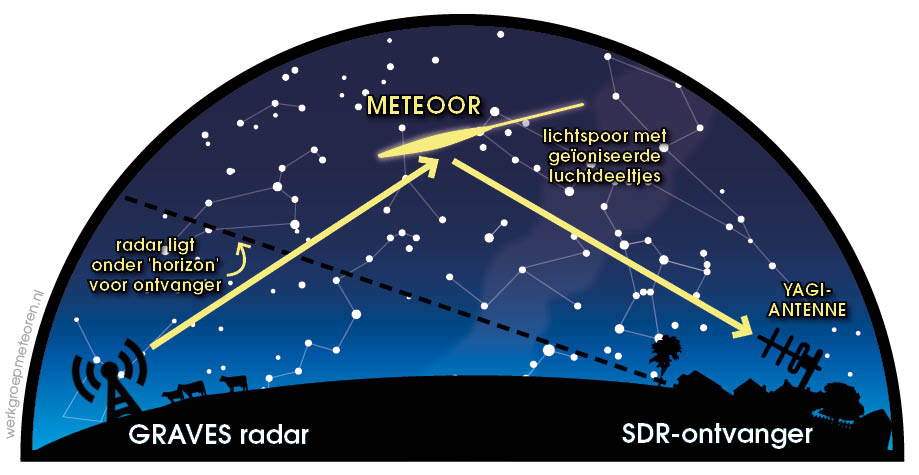
\includegraphics[scale=0.40]{include/figuras/Radar.jpg}
    \caption{Funcionamiento del radar GRAVES}
    \label{fig:radar}
\end{figure}

\vspace{0.5cm}

En el contexto del proyecto se quiere acercar la astronomía a los ciudadanos, ya sean adultos o niños y además hacerla accesible para personas con discapacidad visual. Como parte del proyecto se creará un asistente automatizado apoyado en la inteligencia artificial mediante el cual guiará a los usuarios para ayudarlos a realizar la clasificación de los cuerpos celestes, ya sea a través de escritura o por voz.
Como resultado del proyecto se pretende conseguir una clasificación de los meteoros y contrastarla con las publicadas en artículos científicos.


\section{Objetivos}


La introducción del TFG debe servir para que los profesores que evalúan el Trabajo puedan comprender el contexto en el que se realiza el mismo, y los objetivos que se plantean.

Esta plantilla muestra la estructura básica de la memoria final de TFG, así como algunas instrucciones de formato.

El esquema básico de una memoria final de TFG es el siguiente:
\begin{itemize}
\item[•] Resumen en español y inglés (máximo 2 páginas cada uno)
\item[•] Tabla de contenidos
\item[•] Introducción (con los objetivos del TFG)
\item[•] Desarrollo
\item[•] Resultados y conclusiones
\item[•] Bibliografía (publicaciones utilizadas en el estudio y desarrollo del trabajo)
\item[•] Anexos (opcional)
\end{itemize}

En cualquier caso, es el tutor del TFG quien indicará a su estudiante la estructura de memoria final que mejor se ajuste al trabajo desarrollado.

Con respecto al formato, se seguirán las siguientes pautas, que se muestran en esta plantilla:
\begin{itemize}
\item[•] \textit{Tamaño de papel:} DIN A4
\item[•] \textit{Portada:} tal y como se recoge en esta plantilla, con indicación de universidad, centro, título de TFG y autor.
\item[•] \textit{Segunda página:} información bibliográfica, incluyendo todos los datos del tutor del TFG.
\item[•] \textit{Tipo de letra para texto.} Preferiblemente “Bookman Old Style” 11 puntos. Si no fuera posible, las alternativas recomendadas son, por orden de preferencia: “Palatino Linotype”, “Garamond” o “Georgia”.
\item[•] \textit{Tipo de letra para código fuente:} “Consolas” o “Roboto mono”
\item[•] \textit{Márgenes:} superior e inferior $3$ cm, izquierdo y derecho $2.54$ cm.
\item[•] \textit{Secciones y subsecciones:} reseñadas con numeración decimal a continuación del número del capítulo. Ej.: subsecciones 2.3.1.
\item[•] \textit{Números de página:} siempre centrado en margen inferior, página 1 comienza en capítulo 1, todas las secciones anteriores al capítulo 1 en número romano en minúscula (i, ii, iii…).
\end{itemize}

\vspace*{1.5cm}
Para elaborar la memoria final del TFG con esta plantilla, seguir los siguientes pasos:
\begin{enumerate}
\item Descargar e instalar MiKTeX:  \url{https://miktex.org/}
\item Descargar e instalar un editor de \LaTeX~, por ejemplo Texmaker:\\
\url{https://www.xm1math.net/texmaker/}

\item Editar el archivo \textbf{secciones/ \_DatosTFG.tex}, que hay en la carpeta \textbf{secciones} de esta plantilla. Cumplimentar todos los datos pedidos en dicho archivo. Guardar y cerrar.
\item Compilar el archivo \textbf{plantilla\_TFG.tex} (puede ser renombrado). Se generará como resultado un archivo \textbf{pdf}.
\item Para escribir la memoria final del TFG se pueden añadir y/o modificar los archivos de la carpeta \textbf{secciones} como sea necesario. El resultado se obtiene al compilar el archivo \textbf{plantilla\_TFG.tex}. 
\end{enumerate}

%%---------------------------------------------------------